\documentclass[a4paper, 9pt]{article}

% page layout
\usepackage{geometry}
\geometry{lmargin=1.3in, rmargin=1.3in}

% Allow fancy headers and footers
\usepackage{fancyhdr}
\pagestyle{fancy}
\fancyhf{}

% Show fancy page numbers (X of XX) at the bottom of each page
% If hyperref package is used then starred commands, e.g.
% '\pageref*{}' are available.
\usepackage{lastpage}

% fancy header
\renewcommand{\headrulewidth}{0pt}
\lhead{} 
\chead{}
\rhead{}

% fancy footer
\cfoot{Side \thepage \hspace{1pt} / \pageref*{LastPage}}

% header formatting
\usepackage{sectsty}
\sectionfont{\large}

\usepackage{titlesec}
%% \titleformat{\section}[block]
%%   {\fontsize{12}{15}\bfseries\sffamily\filcenter}
%%   {\thesection}
%%   {1em}
%%   {\MakeUppercase}
%% \titleformat{\subsection}[hang]
%%   {\fontsize{12}{15}\bfseries\sffamily}
%%   {\thesubsection}
%%   {1em}
%%   {}
\titlespacing*{\section}{1pt}{2.0\baselineskip}{0.8\baselineskip}
\titleformat{\section}[block]{\fontsize{19}{30}\Large\bfseries}{\thesection}{1em}{}

% danish letters and text symbols
\usepackage[utf8]{inputenc}
\usepackage[T1]{fontenc}

% links
\usepackage{hyperref}

% images
%\usepackage{float}
\usepackage{graphicx}

% alltt: commands in verbatim
\usepackage{alltt}

% title page
\title{Emacs: C Guide}
\author{Alexander Christensen}

% emacs commands
\newcommand{\key}[1]{\texttt{"#1"}}
\newcommand{\cmd}[1]{\texttt{"#1"}}
\newcommand{\package}[1]{\texttt{'#1'}}
\newcommand{\keycmd}[2]{\key{#1} {\ensuremath\rightarrow} \texttt{"#2"}}
\newcommand{\thenkey}[1]{{\ensuremath\rightarrow} \key{#1}}
\newcommand{\thencmd}[1]{{\ensuremath\rightarrow} \cmd{#1}}
\newcommand{\example}[1]{\vspace{3mm}\noindent\textbf{\underline{\ \ \ \ #1}}\vspace{2mm}\\}

% code formatting
\usepackage{listings}
\usepackage{color}

\definecolor{backgroundblue}{rgb}{0.93, 0.93, 1.0}
\definecolor{mygreen}{rgb}{0,0.6,0}
\definecolor{mygray}{rgb}{0.5,0.5,0.5}
\definecolor{mymauve}{rgb}{0.58,0,0.82}

\definecolor{LightCyan}{rgb}{0.88,1,1}
\definecolor{bluekeywords}{rgb}{0.13,0.13,1}
\definecolor{greencomments}{rgb}{0,0.5,0}
\definecolor{turqusnumbers}{rgb}{0.17,0.57,0.69}
\definecolor{redstrings}{rgb}{0.5,0,0}
\definecolor{red}{rgb}{0.5,0.0,0.0}
\definecolor{blue}{rgb}{0.0,0.5,1.0}
\definecolor{green}{rgb}{0.0,0.5,0.0}

% basic settings, can be overrided
\lstset{
  basicstyle=\ttfamily\small,
  breaklines=true,
  columns=fullflexible,
  escapeinside={\%},
  frame=none,
  backgroundcolor=\color{backgroundblue},
  showspaces=false,
  keepspaces=true,
  showstringspaces=false,
  showtabs=false,
  numbers=left,
  aboveskip=-3pt,
  sensitive=true
}

\lstdefinelanguage{ELisp}
{
language=Lisp,
morekeywords={setq, defun, defvar, eq, when, unless, member},
keywordstyle=\color{bluekeywords},
morecomment=[l][\color{greencomments}]{;},
escapeinside={"},
extendedchars=true,
alsoletter={"},
sensitive=false,
showstringspaces=false,
%stringstyle=\color{redstring},
morestring=[b][\color{redstrings}]",
title={\headline{\small elisp - \textit{\lstname}}},
numbers=none
}

% nice horizontal line "-------- <text> --------", used above a listing
\def\headline#1{\begin{minipage}{36em}\vspace{4mm}\hrulefill\quad\lower.3em\hbox{#1}\quad\hrulefill\end{minipage}}

% horizontal line, used below a listing
\newcommand{\lstline}{\vspace{-3mm}\hrulefill\vspace{2mm}\newline}

% fancy insert listing command
% example of usage: `\customlisting{FSharp}{Some Function}{<file.fsx>}`
\newcommand{\customlisting}[3]{\lstinputlisting[language=#1,name=#2]{#3}\lstline}


\begin{document}
\maketitle

\abstract{\footnotesize\begin{center}
Guide til opsætning af C udviklingsmiljø i Emacs, herunder indentering, kompilering, auto-completion, pakkekonfiguration, samt navigation.\end{center}}


\section{Introduktion}
Denne guide henvender sig primært til studerende på DIKU, som skal til at påbegynde deres andet studieår, og som derfor skal lære at programmere \texttt{C}. Der vil blive lagt væk på pakker og konfigurationer, der knytter sig specifikt til C (eller C++) programmering, og mange fundamentale elementer som fx navigation mellem filer, genvejstaster osv. vil ikke blive berørt.


\section{Notation}
I Emacs jargon betyder \key{C-c} at man trykker "Control c" på sit tastatur, \key{M-c} betyder "Alt c", og \key{RET} betyder "enter". En \texttt{buffer} er en åben instans af en fil, en \texttt{frame} er et programvindue, og en \texttt{frame} kan inddeles i flere \texttt{windows / vinduer}, som er pladsholdere for \texttt{buffere}. Cursoren kaldes for \texttt{point}.


\section{Init-filen}
Kernen omkring Emacs er den utroligt fleksible init-fil. Hvis Emacs åbnes direkte fra en 'frisk' installation ligner det noget, man vil holde sig langt væk fra! Det er meningen, at Emacs skal have en masse pakker installeret, og en rutineret init-fil kommer let op på flere tusind linjer (den kan deles op over flere filer!).

Så hvor finder man sin init-fil? Svaret afhænger af styresystemet. Flere detaljer kan ses på denne hjemmeside: \url{https://www.emacswiki.org/emacs/InitFile}.

\example{nyttig info:}
\key{C-x C-e} i slutningen af en linje eller blok med E-lisp kode vil evaluere denne linje eller blok.\newline
\keycmd{M-x}{eval-buffer}\thenkey{<RET>} vil læse hele init-filen igennem og aktivere (evaluere) alle skrevne konfigurationer. I visse tilfælde er det dog nødvendigt at lukke Emacs og starte det op igen for at se ændringerne - det sker heldigvis ikke særlig ofte.

\vspace{5mm}\noindent
Efter ændringerne i init-filen er evalueret, kan de aktiveres i eksempelvis en C buffer ved at skrive \keycmd{M-X}{c-mode} \thenkey{<RET>}.


\newpage
\section{Pakker}
Pakker til Emacs kan installeres ved at trykke \keycmd{M-x}{list-packages}. Der kan søges efter pakker med \key{C-s} eller \key{C-r}, og hvis \texttt{point} er placeret i starten af linjen for en pakke, kan denne pakke markeres til installation ved at trykke \key{i}, eller markeres til sletning ved at trykke \key{d}. For at udføre alle markerede installationer/afinstallationer tryk \key{x}.\newline

\noindent
For at få mere udbytte af den indbyggede pakke-manager (læs: flere tilgængelige pakker), da kan der med fordel tilføjes \textbf{Melpa}-arkivet til init-filen, som følgende:

\customlisting{ELisp}{init.el}{add-melpa.el}

\noindent
Disse indstillinger bør stå allerøverst oppe i init-filen.


\section{Customization}
I Emacs er der ingen grænser for, hvad der kan ændres på. Et glimrende eksempel er hvis man skriver \keycmd{M-x}{customize-face}\thencmd{all faces}\thenkey{<RET>}: Så kommer der en lang liste frem over alle \texttt{faces} (dvs. farver, skrifttype/størrelser, osv), der kan konfigureres. I Emacs er der ikke noget, der ikke kan konfigureres, og det er ganske sjovt at 'lege med farverne'.\newline

- I stedet for \cmd{all faces} kan man også vælge \cmd{default}: så kan man ændre baggrundsfarven i Emacs.\newline

- Alle \texttt{customizations} man laver bliver automatisk gemt i init-filen når man trykker \textit{'Save for future sessions'}.


\section{Ielm}
\textit{"Inferior Emacs Lisp Mode"}. Her kan man afprøve sproget \textbf{elisp}, som init-filen er skrevet i. Aktiveres ved at skrive \keycmd{M-x}{ielm}\key{<RET>}. Det er en god øvelse, hvis man gerne vil lære at skrive sine egne udvidelser. (det får man brug for, hvis man har anvendt Emacs længe nok!)

\begin{figure}
\centering
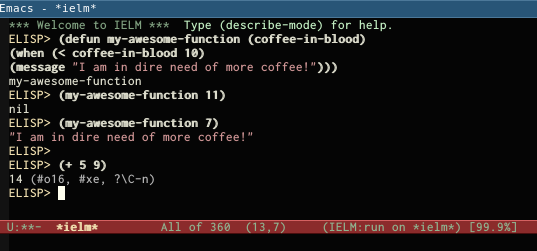
\includegraphics[width=12cm]{ielm-in-action.png}
\caption{\small *Coffee scripting* med \textbf{Ielm}.}
\end{figure}


\newpage
\section{Indentering}
I en aktiv C buffer, tast \key{C-c C-o}, og mini-bufferen vil vise den variabel, som definerer indenteringen på den pågældende linje. Tast \key{RET}, og du har mulighed for at ændre indenteringen (eller tast \key{C-g} for at afbryde).\\

Det er værd at bemærke, at denne indentering er afhængig af, om Emacs er indstillet til at indentere med tabs eller spaces! Til CompSys anbefales det at indentere med 2 spaces, og dette opnås ved at tilføje følende linjer til init-filen:

\customlisting{ELisp}{init.el}{fix-your-indentation.el}

\example{eksempel:}
For at kunne indentere smertefrit med 2 spaces, kunne følgende linjer tilføjes til init-filen:

\customlisting{ELisp}{init.el}{indentation-style.el}

\noindent
Hvis indentering 'driller', brug da metoden vist ovenfor: Undersøg, hvilken variabel, der definerer den pågældende linjes indentering, og tilføj rettelsen til init-filen.


\newpage
\section{Kompilering}
Det kan være et tungt arbejde at kompilere en C fil, især hvis der skal linkes med flere biblioteker, defineres kompiler-version, optimeringsflag, output-fil, etc. Et hårrejsende eksempel på dette kunne være:
\vspace{2mm}\begin{alltt}\footnotesize\centering
gcc -std=gnu11 -Wall -Werror -pedantic -o testfile testfile.c
\end{alltt}\vspace{4mm}

\noindent
Det ville være unødvendigt at skrive dette hver gang i terminalen (selvfølgelig findes der en \texttt{Makefile}!). En hurtig Emacs-løsning ville være følgende tilføjelse til init-filen:

\customlisting{ELisp}{init.el}{my-compile-function.el}

\vspace{-7mm}\begin{center}\footnotesize\texttt{"(interactive)" \textit{betyder i denne sammenhæng at funktionen vil\\ optræde i menuen når man trykker} \key{M-x}}.\end{center}


Det anbefales, at læseren afsætter lidt tid til at forstå, hvordan denne kommando fungerer. Prøv at køre den!


\newpage
\section{Shell-Pop}
Pakken \package{shell-pop} kan være smart hvis man vil hurtigt vil køre en terminalkommando inde fra den mappe, hvori den aktive buffer er hentet fra. Med et tryk på en knap (her er valgt \key{<f2>}) popper der en terminal frem neden under den aktive buffer, og med et tryk på samme knap forsvinder den igen.

\customlisting{ELisp}{init.el}{shell-pop.el}

\noindent
Husk at installere pakken via Emacs' pakke-manager først.

\newpage
\section{Auto-completion}



\newpage
\section{Øvrige referencer}
\url{http://tuhdo.github.io/c-ide.html#sec-2}


\end{document}
